% Options for packages loaded elsewhere
\PassOptionsToPackage{unicode}{hyperref}
\PassOptionsToPackage{hyphens}{url}
%
\documentclass[
]{article}
\usepackage{amsmath,amssymb}
\usepackage{iftex}
\ifPDFTeX
  \usepackage[T1]{fontenc}
  \usepackage[utf8]{inputenc}
  \usepackage{textcomp} % provide euro and other symbols
\else % if luatex or xetex
  \usepackage{unicode-math} % this also loads fontspec
  \defaultfontfeatures{Scale=MatchLowercase}
  \defaultfontfeatures[\rmfamily]{Ligatures=TeX,Scale=1}
\fi
\usepackage{lmodern}
\ifPDFTeX\else
  % xetex/luatex font selection
\fi
% Use upquote if available, for straight quotes in verbatim environments
\IfFileExists{upquote.sty}{\usepackage{upquote}}{}
\IfFileExists{microtype.sty}{% use microtype if available
  \usepackage[]{microtype}
  \UseMicrotypeSet[protrusion]{basicmath} % disable protrusion for tt fonts
}{}
\makeatletter
\@ifundefined{KOMAClassName}{% if non-KOMA class
  \IfFileExists{parskip.sty}{%
    \usepackage{parskip}
  }{% else
    \setlength{\parindent}{0pt}
    \setlength{\parskip}{6pt plus 2pt minus 1pt}}
}{% if KOMA class
  \KOMAoptions{parskip=half}}
\makeatother
\usepackage{xcolor}
\usepackage[margin=1in]{geometry}
\usepackage{longtable,booktabs,array}
\usepackage{calc} % for calculating minipage widths
% Correct order of tables after \paragraph or \subparagraph
\usepackage{etoolbox}
\makeatletter
\patchcmd\longtable{\par}{\if@noskipsec\mbox{}\fi\par}{}{}
\makeatother
% Allow footnotes in longtable head/foot
\IfFileExists{footnotehyper.sty}{\usepackage{footnotehyper}}{\usepackage{footnote}}
\makesavenoteenv{longtable}
\usepackage{graphicx}
\makeatletter
\def\maxwidth{\ifdim\Gin@nat@width>\linewidth\linewidth\else\Gin@nat@width\fi}
\def\maxheight{\ifdim\Gin@nat@height>\textheight\textheight\else\Gin@nat@height\fi}
\makeatother
% Scale images if necessary, so that they will not overflow the page
% margins by default, and it is still possible to overwrite the defaults
% using explicit options in \includegraphics[width, height, ...]{}
\setkeys{Gin}{width=\maxwidth,height=\maxheight,keepaspectratio}
% Set default figure placement to htbp
\makeatletter
\def\fps@figure{htbp}
\makeatother
\setlength{\emergencystretch}{3em} % prevent overfull lines
\providecommand{\tightlist}{%
  \setlength{\itemsep}{0pt}\setlength{\parskip}{0pt}}
\setcounter{secnumdepth}{5}
\newlength{\cslhangindent}
\setlength{\cslhangindent}{1.5em}
\newlength{\csllabelwidth}
\setlength{\csllabelwidth}{3em}
\newlength{\cslentryspacingunit} % times entry-spacing
\setlength{\cslentryspacingunit}{\parskip}
\newenvironment{CSLReferences}[2] % #1 hanging-ident, #2 entry spacing
 {% don't indent paragraphs
  \setlength{\parindent}{0pt}
  % turn on hanging indent if param 1 is 1
  \ifodd #1
  \let\oldpar\par
  \def\par{\hangindent=\cslhangindent\oldpar}
  \fi
  % set entry spacing
  \setlength{\parskip}{#2\cslentryspacingunit}
 }%
 {}
\usepackage{calc}
\newcommand{\CSLBlock}[1]{#1\hfill\break}
\newcommand{\CSLLeftMargin}[1]{\parbox[t]{\csllabelwidth}{#1}}
\newcommand{\CSLRightInline}[1]{\parbox[t]{\linewidth - \csllabelwidth}{#1}\break}
\newcommand{\CSLIndent}[1]{\hspace{\cslhangindent}#1}
\usepackage{fontspec} \setmainfont{Times New Roman} \setmonofont{Arial Unicode MS} \usepackage{lineno} \linenumbers
\ifLuaTeX
  \usepackage{selnolig}  % disable illegal ligatures
\fi
\IfFileExists{bookmark.sty}{\usepackage{bookmark}}{\usepackage{hyperref}}
\IfFileExists{xurl.sty}{\usepackage{xurl}}{} % add URL line breaks if available
\urlstyle{same}
\hypersetup{
  pdftitle={How many speech sounds are there in the world's languages?},
  hidelinks,
  pdfcreator={LaTeX via pandoc}}

\title{How many speech sounds are there in the world's languages?}
\author{Steven Moran\textsuperscript{1,2} \& Nicholas A.
Lester\textsuperscript{3}\\
\textsuperscript{1}Institute of Biology, University of Neuchâtel,
Neuchâtel, Switzerland\\
\textsuperscript{2}Department of Anthropology, University of Miami,
Coral Gables, FL, USA\\
\textsuperscript{3}Department of Linguistics, University of North Texas,
Denton, TX, USA\\
OrcID, SM, 0000-0002-3969-6549\\
Corresponding authors:
\href{mailto:steven.moran@unine.ch}{\nolinkurl{steven.moran@unine.ch}};
\href{mailto:nicholas.a.lester@gmail.com}{\nolinkurl{nicholas.a.lester@gmail.com}}}
\date{04 August, 2023}

\begin{document}
\maketitle

\hypertarget{abstract}{%
\section*{Abstract}\label{abstract}}
\addcontentsline{toc}{section}{Abstract}

How many speech sounds are there in the world's languages? To answer
this question, we extend two formal models of lexical diversity to
segmental phonology. Zipf's law states that most word types are rare;
Herdan-Heaps' law states that vocabulary size grows indefinitely with
increasingly new text. We find that both models produce accurate
estimates of the diversity of contrastive speech sounds (phonemes) in
existing typological databases. Our findings suggest that (a) most
phonemes are difficult to detect because they are rare, and (b)
increased documentation of phonological inventories always yields more
phoneme types. To check this, we apply an unrelated estimator of species
diversity from biology, Chao-Shen, and show that its estimates also
align with Herdan-Heaps' law. We use both models to extrapolate phoneme
counts to undocumented languages, resulting in an estimate of 4600-4900
distinct phonemes in the full set of languages thought to be spoken
today (\textasciitilde7-8k), which is roughly 1.5 time more than what is
currently documented in the world's languages (\textasciitilde35\%). By
extrapolating to hypothetical sample sizes, e.g., the number of
languages estimated to have been spoken through time, and beyond, we
find no indication of convergence: infinite languages mean infinite
phonemes.

\emph{Keywords}: speech, phonetics, phonology, language, Zipf's law,
Herdan-Heaps' law

\begin{center}\rule{0.5\linewidth}{0.5pt}\end{center}

\hypertarget{introduction}{%
\section{Introduction}\label{introduction}}

Under the umbrella of linguistic typology, studies of language diversity
aim to catalog the range of variation in comparable structures across
the world's languages. For some areas of variation, the problem is moot,
i.e., the full range of options is known \emph{a priori}. For example in
grammar, the relative ordering of a verb (V) and its direct object (O)
allows for exactly three possible types: OV, VO, and OV/VO. Thus, every
language falls into one of these categories. Other linguistic domains
are not logically constrained in this way because the true diversity of
types is inherently unknown.

Consider the set of possible speech sounds in the world's languages.
Phonemes are distinguished according to their articulatory, acoustic,
and perceptual properties. However, these properties exist in a
continuous temporal and physical space, which can be carved up in
infinitely many ways. For example, at suitably fine-grained levels of
measurement, no two realizations of the same phoneme will ever be
identical in every dimension of variation.

Thus, each new word presents a non-zero probability of containing a
previously unheard sound, and by extension, new phoneme. Complicating
matters, our current pool of ``consensus phonemes'' -- however defined
-- is subject to re-evaluation in response to advances in data
collection, methods, tools, theories, and experience that inform
language documentation and analysis.\footnote{In the last 20 years or
  so, grammars and phonological descriptions (e.g., \emph{Illustrations
  of the IPA}) increasingly include detailed data and acoustic phonetic
  analysis using software, such as Praat
  (\protect\hyperlink{ref-Boersma2001}{Boersma 2001}). This makes
  phonetic interpretation open to a wider audience.}

The problem is therefore to determine whether there is some sample size
of languages after which no amount of additional phonological
inventories will yield an unseen phoneme type. The absence of a limit
would raise important theoretical issues for the description of
phonemes, including questions concerning the role of phonetics in
phonology (\protect\hyperlink{ref-Whalen2019}{Whalen 2016}) and the
importance of cross-linguistic variation
(\protect\hyperlink{ref-Hockett1963}{Hockett 1963};
\protect\hyperlink{ref-EvansLevinson2009}{Evans \& Levinson 2009}).

The present study seeks to determine whether such a limit exists. To
meet this goal, we propose several methods for modeling the relationship
between sample size and number of linguistic types. We apply these
methods to ask three core questions. First, how many phonemes are there
in the world today (based on a limited sample)? Second, how many
phonemes have there been in the history of human language? And lastly,
how many phonemes are possible in human language? In Section 2, we
motivate our research questions. In Section 3, we describe the data and
in Section 4 we present our methods and results. In Section 5, we
discuss our results and avenues for future research.

\hypertarget{motivation}{%
\section{Motivation}\label{motivation}}

The question of whether there are limits on the number of distinct
speech sounds that can appear in spoken languages has been recognized
for some time. Alexander J. Ellis (1814--1890) stated as early as 1848
that the number of different speech sounds, i.e., candidate phonemes, is
in principle infinite. At that time, teachers and philologists aimed to
develop a transcription standard that could discriminate between all
manners of speech sounds with orthographic symbols for purposes that
included (particularly English) spelling reform and orthography
development for newly documented and unwritten languages (e.g., for
bible translation). But as practitioners increasingly converted the
articulations of more and more languages into a universal phonetic
alphabet, the need for new symbols also seemingly increased without
limit (\protect\hyperlink{ref-Hockett1995-phoneme}{Hockett 1995}, pg.
63).\footnote{This early work later became the basis for the
  International Phonetic Association (and its phonetic alphabet; both
  abbreviated IPA). First published in 1888, today the IPA provides and
  maintains a speech transcriptional device that encodes aspects of
  articulation, and acoustics, for both narrow (phonetic) and broad
  (phonemic) transcription. It is comprised of a set of alphabetic
  symbols and diacritics with the aim of representing all possible
  sounds in the world's spoken languages (there are extensions for
  disordered speech and speech pathology). The IPA provides a summary of
  linguists' phonetic knowledge. This system uses a set of ``base''
  symbols, e.g., letters or combination of letters, that aim to encode
  phonemes, and the use of diacritics on base glyphs to provide phonetic
  detail. Its design also affords infinite transcription possibilities.}
Finer and finer distinctions in phonetic detail created more and more
space for novel phonemes to emerge. Thus, if the phonetic distinctions
to be drawn are infinite, then tautologically so are the number of
possible phonemes.

If there was any doubt about the infinite nature of the speech signal,
instrumental phonetics put the nail in the coffin. Jean-Pierre Rousselot
(1846--1924) studied acoustic properties of speech with the kymograph,
originally developed to measure physiological patterns such as blood
pressure. The later advent of the phonograph by Thomas Edison
(1847--1931) in 1877 provided a means to record and reproduce sound.
Then during WWII the sound spectogram was developed in secret to analyze
ciphony by making sounds visible. The work on visible speech was
released publicly after the war
(\protect\hyperlink{ref-Potter1945}{Potter 1945}) and the spectrogram
became the staple of acoustic phonetic analysis beginning with Joos
(\protect\hyperlink{ref-Joos1948}{1948}) (Joos was the first linguist to
have extensive access to the acoustic spectrograph). For speech, it
measured fluctuations in air pressure, which capture duration, pitch,
and intensity. Thus, the ability to record, measure, and visualize
speech shows that it is dynamic and continuous, even if listeners
perceive it as discrete, e.g., phonemes, syllables, words.\footnote{This
  relationship between continuous and discrete is at the core of the
  debate about the interface between phonetics and phonology
  (\protect\hyperlink{ref-Whalen2019}{Whalen 2016}). The division goes
  back to at least the late 19th century when phoneticians and
  dialectologists including Henry Sweet (1845--1912; 1877) and Jost
  Winteler (1846--1929; 1876) began making a distinction in language
  descriptions between sounds that change the meaning of words and those
  that do not.}

Aside from the acoustic-phonetic argument, evidence for infinite
phonemes comes from studies on the cross-linguistic frequencies of
speech sounds. Early evidence is found in a large cross-linguistic
sample of phoneme inventories, where inventory is understood as the set
of distinctive sounds attested in a language. This sample is described
in the UCLA Phonological Segment Inventory Database (UPSID; Maddieson
(\protect\hyperlink{ref-Maddieson1984}{1984}), Maddieson \& Precoda
(\protect\hyperlink{ref-MaddiesonPrecoda1990}{1990})). Maddieson
(\protect\hyperlink{ref-Maddieson1984}{1984}) created a
genealogically-balanced sample of the world's languages (\emph{n} = 317)
to investigate cross-linguistic properties of phonological systems and
the relationship between aspects such as inventory size, contents, and
structure. Maddieson noticed that certain segments are more or less
likely to be present in inventories regardless of their size. That is,
certain sounds are almost always present and others are almost never
present. In other words, no segment occurs in every language and some
very frequent segments occur in most languages. Moreover, nearly half of
the reported segment types are singletons in the sample, i.e., one-off
language-specific occurrences.\footnote{Whether rare segments occur more
  or less frequently \emph{within} a language is a language-by-language
  research question. See for example Everett
  (\protect\hyperlink{ref-Everett2018}{2018}).} While Maddieson did not
explicitly test for it, his observations fit a well-attested pattern
known as Zipf's law (\protect\hyperlink{ref-Zipf1936}{Zipf 1936};
\protect\hyperlink{ref-Zipf1949}{Zipf 1949}). Zipf's law states that the
frequency distribution of words in a language is inversely proportional
to their frequency rank. The relationship is log-linear: high frequency
words are few in number but account for most of the tokens in a text,
and low frequency words are many, but occur rarely or even just
once.\footnote{Here is a plot showing Zipf's law in the first 10 million
  words in the Wikipedias from 30 different languages:
  \url{https://en.wikipedia.org/wiki/Zipf\%27s_law\#/media/File:Zipf_30wiki_en_labels.png}.}
, Zipf's law states that the frequency of an element \(f(r)\) is
proportional to the inverse frequency rank of that element (modulated by
an exponent \(\alpha\))
(\protect\hyperlink{ref-Piantadosi2014}{Piantadosi 2014}):\footnote{Piantadosi
  (\protect\hyperlink{ref-Piantadosi2014}{2014}) discusses in detail
  that word frequency distributions are not actually as simple as they
  seem according to Zipf's law. For example, semantics affects word
  frequency distributions. Moreover, observations of Zipf's law have
  been obscured by word frequency distribution plots that fail to
  address correlated errors. Zipfian distributions are not unique to
  language. They appear in various aspects of human society, such as
  music and aspects of the internet, as well as in other biological and
  physical systems. Strikingly, power law distributions can arise from
  nearly nothing (\protect\hyperlink{ref-Piantadosi2014}{Piantadosi
  2014: 1121}).}

\[
f(r) \propto \frac{1}{r^\alpha}
\]

The Zipfian distribution characterizes many aspects of language (and
other natural phenomena). Two features make it interesting for our
purposes. First, it describes systems for which most types are rare,
hence difficult to observe. Second, under certain conditions
(\(\alpha \ge 1\)), the Zipf function is non-asymptotic: more types can
always be added at the rank for singletons, and the expected type count
computed. The fact that Maddieson's observations are consistent with the
Zipfian distribution suggests that phoneme types are indeed difficult to
discover (particularly at the fringe) and that there could be some room
left for additional phonemes.

Moran (\protect\hyperlink{ref-Moran2012}{2012}) revisited the frequency
distribution of segments in a larger sample of the world's languages
(\emph{n} = 1780, including UPSID) and showed that the relationship
between cross-linguistic segment frequency follows a similar pattern as
in the Maddieson (\protect\hyperlink{ref-Maddieson1984}{1984}) (\emph{n}
= 317) and Maddieson \& Precoda
(\protect\hyperlink{ref-MaddiesonPrecoda1990}{1990}) (\emph{n} = 451)
UPSID language samples. That is, some phonemes are very frequent across
the world's languages, and half of all documented phonemes are
language-specific. Moran (\protect\hyperlink{ref-Moran2012}{2012}) also
did not explicitly test whether cross-linguistic phoneme frequency
adheres to a Zipfian distribution,\footnote{Moran
  (\protect\hyperlink{ref-Moran2012}{2012}), p.~212 does provide a
  log-log plot of segment frequencies that is Zipfian-esque.} but he
does show that the cumulative number of segment types seems to be
bounded to infinity; the curve appears quadratic and showing no sign of
a slowing towards an asymptote.

In Figure 1, we reproduce these plots using the genealogically balanced
UPSID-451 language sample
(\protect\hyperlink{ref-MaddiesonPrecoda1990}{Maddieson \& Precoda
1990}) and compare it to the data available in the latest version of
PHOIBLE Online (\protect\hyperlink{ref-MoranMcCloy2019}{Moran \& McCloy
2019}), which contains 2186 languages.\footnote{Note that although
  nearly half of the segments in the language samples occur in
  particular languages, some languages contain more than one segment not
  found in any other languages in the sample. This is most apparent from
  the rich phonological inventory of Juǀʼhoan (ISO 639-3: ktz;
  Glottocode: juho1239; aka !Xu, ǃXun, Southeastern ǃKung), which has
  been described as having 141 phonemes -- 66 of which occur in no other
  documented language (\protect\hyperlink{ref-Snyman1970}{Snyman 1970};
  \protect\hyperlink{ref-Snyman1975}{Snyman 1975};
  \protect\hyperlink{ref-MaddiesonPrecoda1990}{Maddieson \& Precoda
  1990}).}

\begin{figure}

{\centering 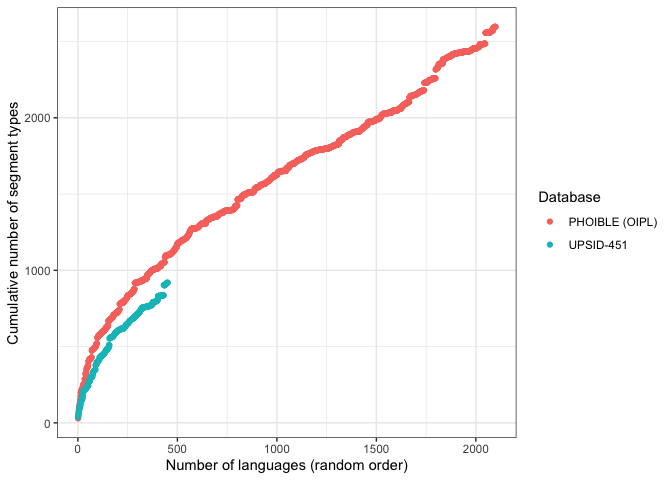
\includegraphics[width=0.8\linewidth]{README_files/figure-gfm/cumulative_plot_phoible_upsid-1} 

}

\caption{Cumulative segments in PHOIBLE 2.0 and UPSID-451}\label{fig:phoible_upsid}
\end{figure}

These plots resemble the distribution of another, less-commonly known
linguistic law: Herdan's and/or Heaps' law. Originally proposed by
Gustav Herdan (\protect\hyperlink{ref-Herdan1964}{1964}), but frequently
attributed to Harold Heaps (\protect\hyperlink{ref-Heaps1978}{1978}) in
the information retrieval literature
(\protect\hyperlink{ref-Egghe2007}{Egghe 2007}), Herdan-Heaps' law
describes the number of distinct words within a document as a function
of the document's (or combined documents') length in terms of total word
count. More specifically, Herdan--Heaps' law states that, as more of a
text is consumed, the rate of never-before-seen words per unit
diminishes (but does not reach 0). This makes intuitive sense given what
we know from Zipf's law: most words are hard to find, and most of the
words that you can find, you have seen before. In fact, Herdan--Heaps'
and Zipf's laws have been shown to be asymptotically equivalent with
respect to individual word frequencies within corpora
(\protect\hyperlink{ref-BaezaNavarro2000}{Baeza--Yates \& Navarro 2000};
\protect\hyperlink{ref-vanLeijenhorst2005}{Leijenhorst \& Van der Weide
2005}). Both of these laws are instances of the same fundamental
property: token counts can be inferred from type counts and vice versa
(\protect\hyperlink{ref-Milivcka2009}{Milička 2009}).

Herdan-Heaps' is expressed as:

\[
V_{R}(n)=Kn^{\beta }
\]

where \(V_{R}\) is the number of distinct words in a text of size
\emph{n} and \emph{K} and \(\beta\) are the free parameters that are
determined empirically. An illustration of a typical Herdan-Heaps' curve
for English text is given in Figure 2 (compare to Figure 1 above).

\begin{figure}

{\centering 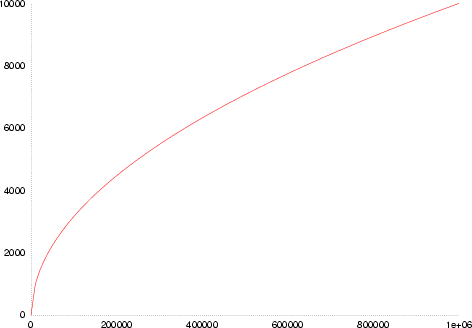
\includegraphics[width=0.8\linewidth]{figures/Heaps_law_plot} 

}

\caption{A typical Herdan-Heaps plot, where x-axis denotes text size and the y-axis the number of distinct vocaulary items (Source: Wikipedia).}\label{fig:heaps}
\end{figure}

Herdan--Heaps' law has been validated using large corpora of naturally
occurring discourse. For example, in a corpus of 50 million words,
Kornai (\protect\hyperlink{ref-Kornai2002}{2002}) found that iteratively
adding more text always led to the discovery of more unique words.
Brants \& Franz (\protect\hyperlink{ref-BrantsFranz2006}{2006}), using a
custom one-trillion-word corpus of English, showed that even with nearly
14 million word types, the growth in vocabulary showed no sign of
stopping.\footnote{Note that ``words'' at the trillion-word scale corpus
  include all segmentable substrings, including alternate spellings for
  the same target word. These alternatives can be numerous. For example,
  Google's spell correction system has detected nearly 600 different
  spellings for the query \emph{britney spears}:
  \url{http://archive.google.com/jobs/britney.html}.}

We can apply the same approach to phonemes nested within inventories. By
analogy to words and documents, phonemes are the words, and the
concatenated inventories of a sample of languages (\emph{L}) is a
document. The ``document'' is expanded by considering new, entire
phoneme inventories one language at a time. Any new phonemes are added
to the existing set and the new count recorded (as in Figure 2 above).
If the phoneme type counts predicted by Herdan-Heaps' law match those of
the known sample of inventories, we can then extrapolate the trend to
larger number of inventories. For example, how many phonemes potentially
exist in the full (but only partially documented) set of the world's
7151 spoken languages.\footnote{This estimate is taken from Ethnologue (
  \url{https://www.ethnologue.com/guides/how-many-languages}?).} What
about even more languages? How many phonemes may have existed throughout
time? And what is the upper bound on the number of distinct phonemes? Is
there one? Or does Herdan--Heaps' law suggest that the number of
phonemes in languages is potentially infinite?

\hypertarget{data}{%
\section{Data}\label{data}}

For this study, we use the latest PHOIBLE data, which includes 3020
phonological inventories from 2186 distinct languages, covering 3183
distinct phonemes (\protect\hyperlink{ref-MoranMcCloy2019}{Moran \&
McCloy 2019}). The dataset is a convenience sample of languages, in
which some geographic regions and language families have greater or
lesser coverage. Included in PHOIBLE is UPSID-451
(\protect\hyperlink{ref-Maddieson1984}{Maddieson 1984};
\protect\hyperlink{ref-MaddiesonPrecoda1990}{Maddieson \& Precoda
1990}), a genealogically balanced sample of languages in which each data
point was selected as a representative of its language family.
Therefore, we use both UPSID and PHOIBLE as baselines to evaluate our
models.

Our central question concerns how the number of spoken languages that
are documented relate to the number of unique phonemes that are
observed. This is a question of cumulative growth. It can be rephrased
as: if we have seen \emph{x} languages with \emph{y} unique phonemes,
how many unique phonemes do we expect to find in \(x + i\) languages?

\hypertarget{methods-and-results}{%
\section{Methods and results}\label{methods-and-results}}

\hypertarget{zipfs-law}{%
\subsection{Zipf's law}\label{zipfs-law}}

First, we test whether the segment distribution in the databases follow
\href{https://en.wikipedia.org/wiki/Zipf\%27s_law}{Zipf's law}. Figures
3 \& 4 plot log frequency (y-axis) by log frequency rank (x-axis) for
UPSID and PHOIBLE, respectively. The circles represent the cumulative
distributional counts of each phoneme. The blue dotted line represents
predictions based on Zipf's distribution using the following equation:

\[
\begin{aligned}
  f(rank;a;b;c) & = \log{\frac{c}{(rank+b)^a}} \\ 
  &= \log{(c) + a \cdot\log{(rank + b)}}
\end{aligned}
\]

where \(a\), \(b\), and \(c\) are tunable parameters. In this case, we
determined the optimal parameters using non-linear least squares
regression as implemented in the \emph{nls} function from the
\emph{stats} package (v. 3.6.2) for the programming environment \emph{R}
(\emph{R} Core Team, 2019).

\begin{figure}

{\centering 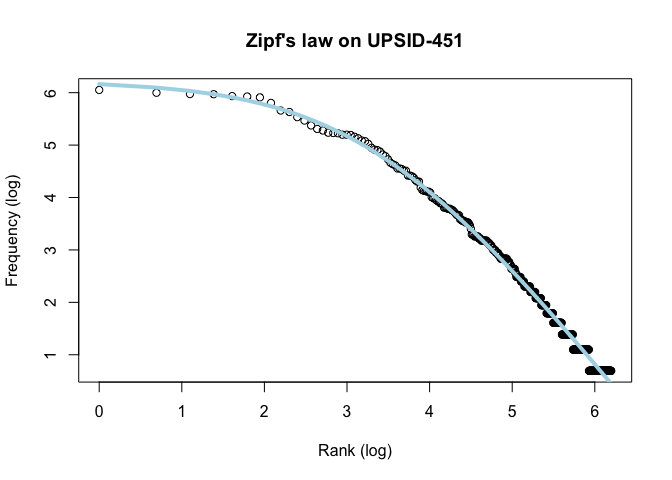
\includegraphics[width=0.8\linewidth]{README_files/figure-gfm/zipf_distribution_upsid-1} 

}

\caption{\label{fig:upsid}Cumulative segments in UPSID-451 follow Zipf's law}\label{fig:upsid_zipf}
\end{figure}

\begin{figure}

{\centering 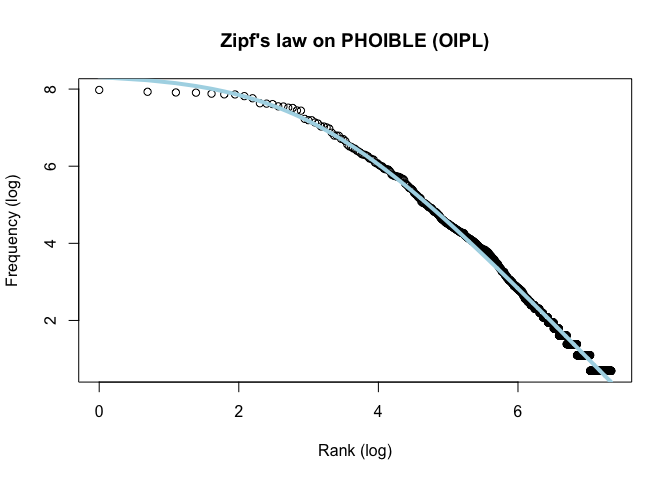
\includegraphics[width=0.8\linewidth]{README_files/figure-gfm/zipf_distribution_phoible-1} 

}

\caption{Cumulative segments in PHOIBLE (OIPL) follow Zipf's law}\label{fig:phoible_zipf}
\end{figure}

The close fit between the observed curve and the predictions drawn from
a Zipfian distribution suggests that global phoneme distributions are
Zipf-distributed.\footnote{We note the debates in the literature on what
  the underlying distributions are of phoneme inventory size (e.g.,
  Lehfeldt (\protect\hyperlink{ref-Lehfeldt1975}{1975}), Justeson \&
  Stephens (\protect\hyperlink{ref-JustesonStephens1984}{1984}),
  Maddieson (\protect\hyperlink{ref-Maddieson2008}{2008})) and of
  phonemes frequencies in text
  (\protect\hyperlink{ref-Martindale_etal1996}{Martindale et al. 1996};
  \protect\hyperlink{ref-TambovtsevMartindale2007}{Tambovtsev \&
  Martindale 2007};
  \protect\hyperlink{ref-Macklin-CordesRound2020}{Macklin-Cordes \&
  Round 2020}). But here we are specifically looking at presence of
  phonemes in phonological inventories cross-linguistically.} Note that
this close approximation holds for both the genealogically balanced and
large-scale databases.

\hypertarget{herdanheaps-law}{%
\subsection{Herdan--Heaps' law}\label{herdanheaps-law}}

The distribution of phonemes in both language samples are clearly
Zipfian. We next test whether their distributions likewise follow
Herdan--Heaps' law. Does the number of yet-to-be-seen segment types
decrease as the number of phonological inventories observed increases by
way of a power law relation?

An important feature of the Herdan-Heaps' equation is that it can be
expressed in the form of a standard linear equation by simply taking the
logarithm of each term, or:

\[
\begin{aligned}
  \log d & = \log (K + n^B)\\
  & = \log K + B \cdot \log n
\end{aligned}  
\]

which has the familiar form:

\[y = \beta_0 + \beta_1 \cdot x\]

This gives us the added benefit of being able to fit a log-transformed
linear regression model to the data, such that:

\begin{itemize}
\tightlist
\item
  The resulting intercept is the optimal \(K\) (with some
  back-transformation: \(K = e^k\)).
\item
  The coefficient \(\beta_1\) expresses \(B\).
\end{itemize}

With these values, we can estimate the type count for any sample size
\(n\) using the standard Herdan-Heaps' equation. As proof of concept, we
estimate the number of phonemes for both UPSID-451 and PHOIBLE. Some
languages in PHOIBLE are associated with more than one doculect. To
avoid an overrepresentation bias, we randomly sample one doculect from
every language or take the single doculect where only one exists (one
inventory per language, or OIPL. Results of a preliminary analysis
indicated that the full and OIPL versions of PHOIBLE behaved similarly.
We therefore focus on the results from the OIPL database here (see the
supplementary materials for comparisons between the full and OIPL
versions).

We begin by randomly permuting the order of inventories and computing
the cumulative number of unique segment types for each new language
observed. Then we repeat this process \(k\) times (we set k=10 trials)
for each database. We fit a log-linear regression to the resulting sets
of estimates to generate empirically optimal values for \(B\) and \(K\)
-- our two free parameters in the Herdan-Heaps' equation.

Figures 5, 6 \& 7 show the predicted values against the true values of
the number of segment types (phoneme type count) versus segments
recorded in phonological inventories in the samples (segment token
count). Model fits for the UPSID-451 and PHOIBLE language samples
suggest that the phoneme type versus token count closely follows
Herdan-Heaps' law.\footnote{In the supplementary materials, we also fit
  a ``one inventory per language'' (OIPL) model of PHOIBLE to show that
  the language sample's genealogical and areal biases, e.g., the sample
  is more representative of African languages than other world areas,
  are not affected by simply sampling the whole database. The outcomes
  between a stratified random resampling and testing the segment type
  versus token on the entire convenience sample are nearly the same.}

\begin{figure}

{\centering 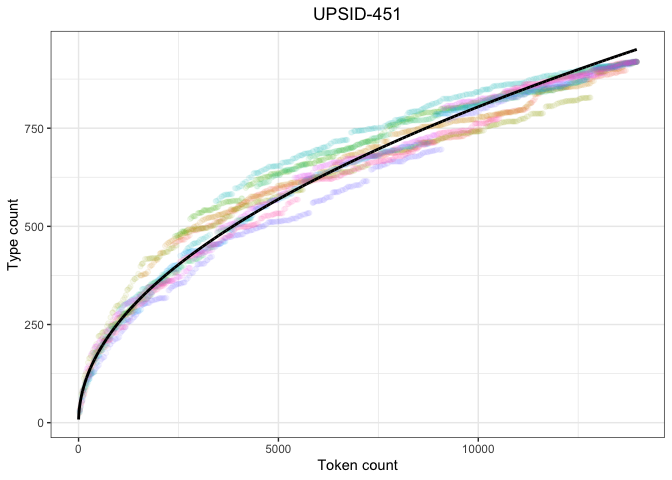
\includegraphics[width=0.8\linewidth]{README_files/figure-gfm/heaps_upsid-1} 

}

\caption{\label{fig:upsid}Cumulative segments in UPSID-451 follow Zipf's law}\label{fig:upsid_heaps}
\end{figure}

\begin{figure}

{\centering 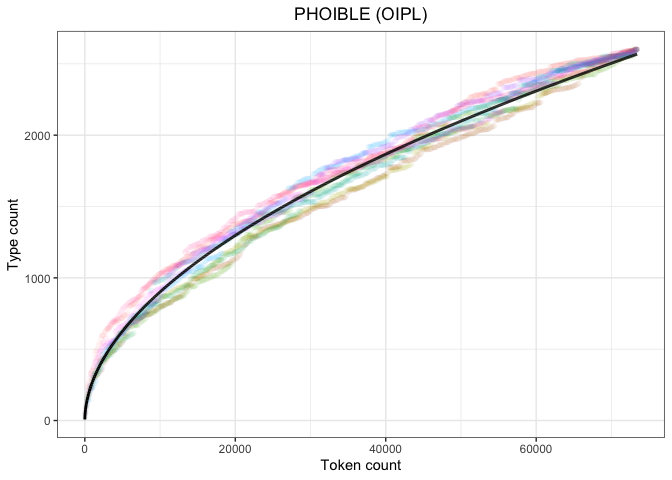
\includegraphics[width=0.8\linewidth]{README_files/figure-gfm/heaps_phoible_oipl-1} 

}

\caption{\label{fig:upsid}: Cumulative segments in PHOIBLE (OIPL) follow Zipf's law}\label{fig:phoible_heaps}
\end{figure}

Next, we compare the model parameters across the two databases,
UPSID-451 and PHOIBLE. The values for \(B\) and \(K\) are relatively
similar. UPSID-451 and PHOIBLE (all) have nearly identical values for B,
but they differ in the scalar K, which explains the sharper increases in
segment type counts for PHOIBLE.

\begin{longtable}[]{@{}lll@{}}
\toprule\noalign{}
Database & B & K \\
\midrule\noalign{}
\endhead
\bottomrule\noalign{}
\endlastfoot
UPSID & 0.4994352 & 8.087208 \\
PHOIBLE (OIPL) & 0.5442040 & 5.870403 \\
\end{longtable}

We illustrate these parameter differences in Figure 7 by combining the
plots on the same scale. The curve describing Herdan-Heaps' estimates
based on UPSID-451 has a shallower trajectory than the curve based on
PHOIBLE. Nevertheless, both curves are highly similar. This similarity
indicates that the known areal and genetic biases present in PHOIBLE do
not have much of an effect on the modeling of phoneme diversity. Based
on this finding, we focus on the larger and more complete database,
PHOIBLE, in the remaining analyses.

\begin{figure}

{\centering 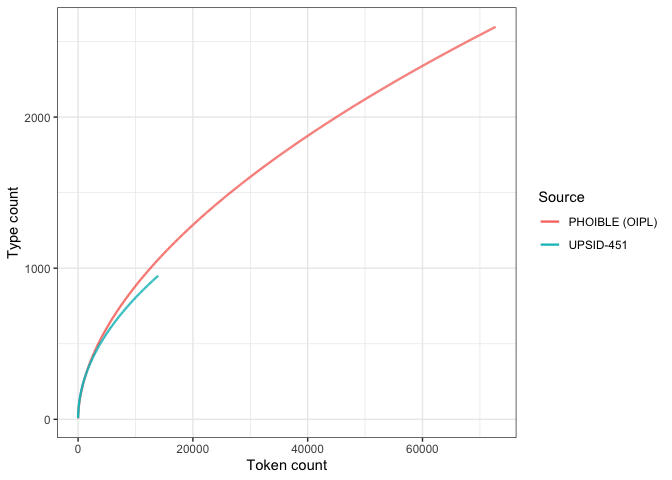
\includegraphics[width=0.8\linewidth]{README_files/figure-gfm/compare_models-1} 

}

\caption{\label{fig:upsid}: Cumulative segments in UPSID-451 and PHOIBLE (OIPL) follow Herdan-Heaps' law}\label{fig:compare_models}
\end{figure}

Next, we implement a general and flexible estimator for type counts
called the Chao-Shen estimator
(\protect\hyperlink{ref-Chao_etal2009}{Chao et al. 2009};
\protect\hyperlink{ref-ChaoChiu2016}{Chao \& Chiu 2016}). If the results
from the two estimators (Chao-Shen and Herdan-Heaps' law) converge, then
we have a more solid foundation for extrapolating phoneme counts for
larger, hypothetical sample sizes.

\hypertarget{the-chao-shen-estimator}{%
\subsection{The Chao-Shen estimator}\label{the-chao-shen-estimator}}

The Chao-Shen estimator was developed to determine the diversity of
species within an ecosystem given only limited (spatial and temporal)
sampling (\protect\hyperlink{ref-Chao_etal2009}{Chao et al. 2009};
\protect\hyperlink{ref-ChaoChiu2016}{Chao \& Chiu 2016}). It allows us
to extrapolate the number of types in some population based on an
incomplete sample using the number of rare types and an estimate of the
number of unobserved types.

This estimator takes as input an incidence matrix and returns the
expected number of types in a larger (imaginary) sample. An incidence
matrix is a record of the presence or absence of the types being sampled
from a set of sampling units. For example, imagine that an entomologist
is interested in identifying how many types of beetles are in a forest.
She knows from prior research that there are 1000 documented species of
beetles in the area. In order to get a representative sample of the
diversity of beetle species in the overall ecosystem, she sets up 50
beetle traps, regularly spaced across the forest. In this example, the
traps are the sampling units and the species of beetles are the types.
The entomologist prepares a 50 X 1000-cell spreadsheet in which the rows
and columns correspond to the traps and known beetle species,
respectively. She then visits each trap and for each of the 1000 known
species of beetle she finds, she records a 1 for that species in
appropriate cell. All unseen species are given a value of 0. The result
after all traps have been visited is a 50 X 1000 incidence matrix. The
information contained in this matrix can then be fed into the Chao-Shen
estimator to provide an estimate of the true diversity of beetle species
in the forest.

The same approach can be extended to languages and their phonemes. On
analogy with the beetle example, the forest is the sum of the
human-populated areas of Earth; the beetle traps are all documented
human languages; and the beetles are the phonemes which appear in those
languages. The incidence matrix is of shape \emph{l} X \emph{s}, where
\emph{l} is the number of documented languages and \emph{s} is the
number of types of segments that have been documented as phonemes in at
least one language. By definition, if a segment appears as a phoneme in
a given language, the corresponding cell in the incidence matrix
contains a 1; otherwise, it contains a 0.

Table 1 shows a hypothetical example of an incidence matrix for 150
observed segments from a set of \(S_{obs}\) phonemes in \(R\) languages.
Marginal sums are given per language (\(\sum_{language}\), or
\emph{inventory size}) and per segment (\(\sum_{phoneme}\), or
\emph{cross-linguistic prevalence})

\begin{longtable}[]{@{}
  >{\centering\arraybackslash}p{(\columnwidth - 10\tabcolsep) * \real{0.2273}}
  >{\raggedright\arraybackslash}p{(\columnwidth - 10\tabcolsep) * \real{0.1364}}
  >{\raggedright\arraybackslash}p{(\columnwidth - 10\tabcolsep) * \real{0.1364}}
  >{\centering\arraybackslash}p{(\columnwidth - 10\tabcolsep) * \real{0.2273}}
  >{\raggedright\arraybackslash}p{(\columnwidth - 10\tabcolsep) * \real{0.1364}}
  >{\raggedright\arraybackslash}p{(\columnwidth - 10\tabcolsep) * \real{0.1364}}@{}}
\caption{Hypothetical sample of an incidence matrix}\tabularnewline
\toprule\noalign{}
\begin{minipage}[b]{\linewidth}\centering
Phoneme
\end{minipage} & \begin{minipage}[b]{\linewidth}\raggedright
Lang1
\end{minipage} & \begin{minipage}[b]{\linewidth}\raggedright
Lang2
\end{minipage} & \begin{minipage}[b]{\linewidth}\centering
···
\end{minipage} & \begin{minipage}[b]{\linewidth}\raggedright
Lang\emph{R}
\end{minipage} & \begin{minipage}[b]{\linewidth}\raggedright
∑phoneme
\end{minipage} \\
\midrule\noalign{}
\endfirsthead
\toprule\noalign{}
\begin{minipage}[b]{\linewidth}\centering
Phoneme
\end{minipage} & \begin{minipage}[b]{\linewidth}\raggedright
Lang1
\end{minipage} & \begin{minipage}[b]{\linewidth}\raggedright
Lang2
\end{minipage} & \begin{minipage}[b]{\linewidth}\centering
···
\end{minipage} & \begin{minipage}[b]{\linewidth}\raggedright
Lang\emph{R}
\end{minipage} & \begin{minipage}[b]{\linewidth}\raggedright
∑phoneme
\end{minipage} \\
\midrule\noalign{}
\endhead
\bottomrule\noalign{}
\endlastfoot
\textbf{Phon1} & 1 & 0 & ··· & 0 & 1 \\
\textbf{Phon2} & 0 & 1 & ··· & 1 & 2 \\
··· & ··· & ··· & ··· & ··· & ··· \\
\textbf{Phon\emph{S}obs} & 1 & 1 & ··· & 1 & 30 \\
\textbf{∑language} & 15 & 23 & ··· & 6 & 150 \\
\end{longtable}

Using the definitions provided above, the Chao-Shen estimator is
expressed formally as follows:

\[ \hat{S}_{\text{Chao-Shen}} = S_{\text{obs}} + \hat{Q}_0 \left[1 - \left(1 - \frac{Q_1}{Q_1 + R \cdot \hat{Q}_0}\right)^r\right] \]

\(S_{obs}\) is the number of segment types that have been observed
overall. \(R\) is the number of languages in the observed sample.
\(Q_1\) is the number of segment types that have only been observed once
(\emph{singletons}), e.g., Phon1 in Table 1). The hyperparameter \(r\)
expresses the number of new languages that we wish to add
(hypothetically) to our existing sample. Finally, \(\hat{Q}_0\) is the
estimated number of unobserved types that were nevertheless ``truly''
present. We do not have empirical access to this figure -- we cannot
directly measure how much we haven't seen. Therefore, it must be
inferred. \(\hat{Q}_0\) can be derived in many ways. Here, we use the
following equation.

\[ \hat{Q}_0 = \begin{cases} S_{\text{obs}} + \left[\frac{R-1}{R}\right] \frac{Q^2_1}{2 \cdot Q_2} & \text{if }Q_2 > 0 \\ S_{\text{obs}} + \left[\frac{R-1}{R} \right] \cdot Q_1 \cdot \frac{Q_1-1}{2} & \text{if }Q_2 = 0\end{cases}\]

In this equation, \(Q_2\) stands for number of segment types which were
observed exactly twice, or \emph{duplicates} (e.g., Phon2 in Table 1).

Similar to the Herdan-Heaps' equation, we can test how well the
estimates of the model match known values based on increasing sample
sizes. However, unlike Herdan-Heaps', the Chao-Shen estimator requires a
hyperparameter that stipulates how many \emph{additional} observations
it should consider in making its estimate. It looks ahead to larger
samples, rather than at the current sample size. We must therefore
approach this problem differently. Our solution is to sample repeatedly
from our set of languages, each time increasing the number of languages
\(R\) by an increment of \(d\). For each value of \(R\), we compute the
Chao-Shen estimates for several values of \(r\), each time increasing
\(r\) by \(c\) additional observations.

The entire procedure is thus:

\begin{enumerate}
\def\labelenumi{\arabic{enumi}.}
\tightlist
\item
  Pick a random set of phonological inventories of size \(R_s\)
\item
  Compute the frequency vector of the segment types
\item
  Apply the Chao-Shen estimator for \(r\) with \(R = R_s\) 3a. Increase
  \(r\) by \(c\) 3b. Repeat 3a until maximum \(r_{\text{max}}\) is
  reached
\item
  Repeat steps 1-3 \(k\) times 5a. Increase \(R_s\) by \(d\)
\end{enumerate}

Figure 8 shows the results of applying this procedure to PHOIBLE. \(k\)
is arbitrarily set to 10 iterations. The relatively small degree of
variation across iterations suggests that this value is suitably high.
\emph{d} was set to 10. \emph{r} was manually adjusted to exemplify
behavior at different scales (within the limits afforded by the overall
sample size). Grey lines represent the Chao-Shen estimates for each
iteration, and blue lines give the means. Red lines represent the mean
of the true number of observed types across iterations. Red lines become
shorter as \emph{r} increases because we have fewer true values to
compare against when we look further ahead from any position (i.e.,
fewer values of \emph{R} for which we can look \emph{r} steps ahead).

\begin{figure}

{\centering 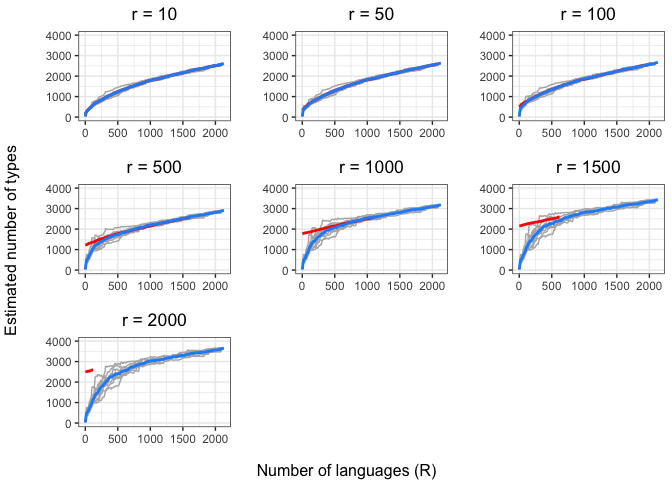
\includegraphics[width=0.8\linewidth]{README_files/figure-gfm/chao_lang_types-1} 

}

\caption{\label{fig:chao_lang_types}Estimated segment types by number of languages}\label{fig:chao_lang_types}
\end{figure}

The first thing to notice about these plots is that they closely
resemble the Herdan-Heaps' curve that we generated from PHOIBLE. These
plots thus also point to slowing but non-asymptotic growth of type
counts.

Regarding the behavior of the parameters, the Chao-Shen estimator shows
near-perfect prediction across values of \emph{R} when \emph{r} is
relatively small. That is, the model is very good at predicting known
segment type counts for samples with relatively fewer additional
languages (small \emph{r}), regardless of the number of observed
languages (all \emph{R}). If we compare the panels against one another,
particularly at lower values of \emph{R}, we see that the differences
between the true values (red lines) and the estimated values (blue
lines) increase with \emph{r}. As \emph{r} increases, so does the degree
of underestimation. In other words, the model is more conservative in
its guesses when data are sparse and the distances of extrapolation are
large. The underestimation appears to dissipate around \emph{R} = 1000.
Figure 9 plots this relationship directly.

\begin{figure}

{\centering 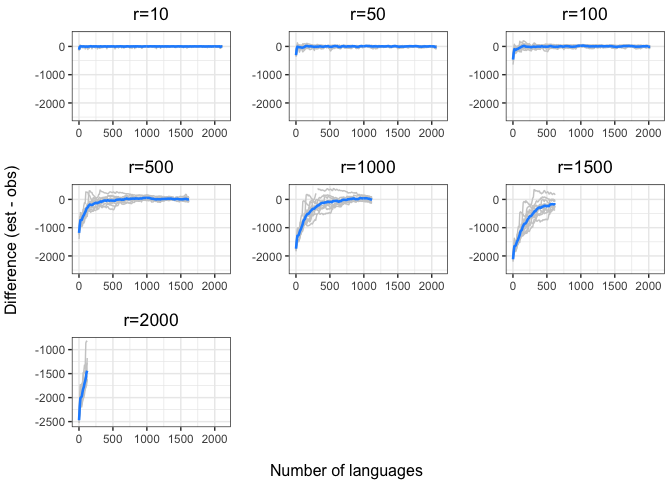
\includegraphics[width=0.8\linewidth]{README_files/figure-gfm/chao_error_estimates-1} 

}

\caption{\label{fig:chao_error_estimates}Chao error estimates in PHOIBLE}\label{fig:chao_error_estimates}
\end{figure}

Variability across iterations increases with \emph{r}, particularly for
sample sizes of \textasciitilde1700 languages or fewer. This pattern
indicates that larger values of \emph{r} should be compensated for by
larger values of \emph{R}. Otherwise, the results may not generalize
well to other samples (even if the other samples are drawn from the same
underlying pool, as we have shown here!).

To summarize, estimates converge on the observed values earlier on
average when \emph{R} is larger relative to \emph{r}. Thus, we do better
when we have more data and predict values closer to our observed sample.
In addition, the variability in estimates across iterations (grey lines)
increases with \emph{r} and decreases with \emph{R}. Thus, our estimates
are noisier when we look further ahead and have smaller samples.
Together these findings suggest two things: (a) the ratio of observed
sample size to sample size increase \(\frac{R}{r}\) should be maximized
to reduce sample-induced noise, and (b) \emph{R} should be maximized to
fight the underestimation bias.

Unfortunately, PHOIBLE offers a proportionally small \emph{R} given some
of the values of \emph{r} that we would like to investigate. For
example, to account for the estimated number of current languages, we
would need \emph{r} = 7151 - 2099 = 5052, a value almost 2.5 times as
large as our observed \emph{R} (2099). Extrapolating from our known
sample to the estimated number of world languages therefore requires an
undesirably small proportion \(\frac{R}{r}\) -- around 0.42. That said,
our data suggest that sample sizes of \textasciitilde1000 languages
produce estimates that closely approximate the true segment type counts,
even as \emph{r} increases. In other words, after 1000 languages,
increases in \emph{R} do less to mitigate the underestimation bias.
Given that PHOIBLE contains more than double that number of languages,
we have no reason to suspect significant underestimation for the
relatively large values of \emph{r} that we investigate here. However,
because of the small ratio of \emph{R}:\emph{r}, we should expect our
estimate to come with greater uncertainty.

We have so far described the distributional properties of our databases,
associated their behavior with two linguistic laws, and introduced two
methods for inferring type counts from an observed frequency
distribution. We now explore in more detail how well the two type
estimators -- Herdan-Heaps' and Chao-Shen -- perform when predicting the
total segment type diversity of a database from an incomplete subsample.

\hypertarget{predicting-known-segment-type-diversity}{%
\subsection{Predicting known segment type
diversity}\label{predicting-known-segment-type-diversity}}

To establish whether we can reliably estimate the number of segment
types in a known sample, we evaluate the accuracy of each estimator in
predicting the known type count given a fixed-size random subsample.
From PHOIBLE (\emph{n} = 2099), we randomly select 1500 languages -- an
arbitrary number that includes roughly three-quarters the number of
languages in the total sample. Note that this value was set above the
threshold of \emph{R} = 1000 (reported above for the Chao-Shen
estimator) to help support prediction accuracy. We then extrapolate our
model parameters from this random sample and use them to predict total
segment type diversity in PHOIBLE. We iterate this process \emph{k} =
100 times.

The Herdan-Heaps' estimates are visualized in Figure 10. The mean is
plotted as a solid black line. The 97.5\% confidence intervals (CIs) are
plotted as dotted lines around the mean. The red dotted line indicates
the true number of phoneme types. Blue shading indicates the density
function of the estimated values from the 100 iterations.

For this run of 100 iterations, the Herdan-Heaps' estimator
overestimated the true value by \textasciitilde18 segment types on
average (\textasciitilde2613 estimated vs.~2596 observed).

\begin{figure}

{\centering 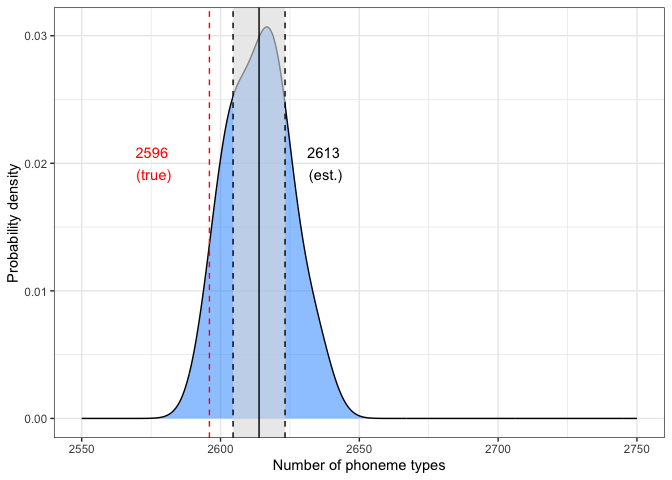
\includegraphics[width=0.8\linewidth]{README_files/figure-gfm/herdan_heaps_ci-1} 

}

\caption{\label{fig:herdan_heaps_ci}Herdan-Heaps' confidence intervals for a sample of 1500 languages}\label{fig:hh_ci}
\end{figure}

Next we test the Chao-Shen estimator. We again sample 1500 languages 100
times from PHOIBLE. The results are plotted in Figure 11.

\begin{figure}

{\centering 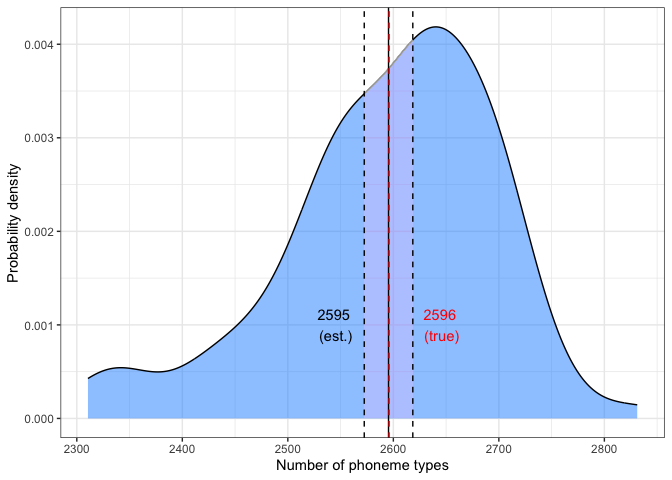
\includegraphics[width=0.8\linewidth]{README_files/figure-gfm/chao_ci-1} 

}

\caption{\label{fig:chao_ci}Chao confidence intervals on a sample for 1500 languages}\label{fig:chao_ci}
\end{figure}

The Chao-Shen estimator overestimates the true value by only 1 type (the
estimate is actually closer: 0.56 types). It therefore provides an
almost perfect fit. Note that \(\frac{R}{r} = \frac{1000}{1099} = 0.91\)
(three times the size of what we face with our extrapolation to the
world's 7151 known languages).

The Chao-Shen estimator therefore seems to outperform Herdan-Heaps' law
in predicting type counts in PHOIBLE. However, we stress that
predictions from both models fall remarkably close to the true value.

As a final point of comparison, we plot Herdan-Heaps estimates against
the corresponding Chao-Shen estimates for increasing sample size and
values of \emph{r} (Figure 12).

\begin{figure}

{\centering 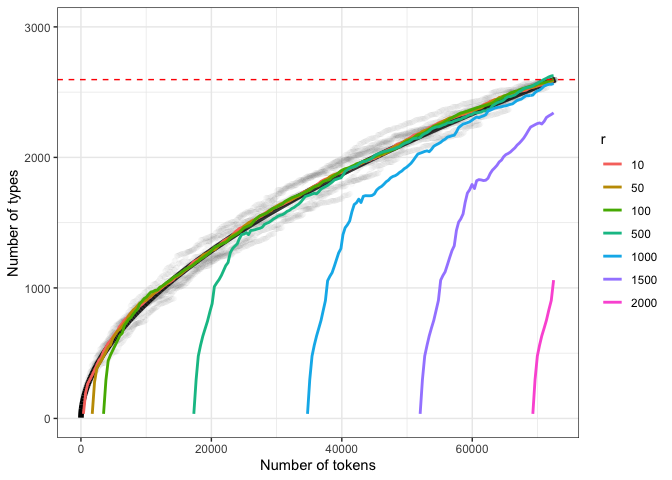
\includegraphics[width=0.8\linewidth]{README_files/figure-gfm/comp_plot-1} 

}

\caption{\label{fig:comp_plot}Comparing the Herdan-Heaps' and Chao esimtator}\label{fig:comp_plot}
\end{figure}

The black line represents PHOIBLE-based Herdan-Heaps estimates. Grey
points reflect true cumulative type counts from 10 reshuffled versions
of PHOIBLE. The horizontal dotted red line indicates the total known
number of segment types in PHOIBLE. The solid colored lines represent
Chao-Shen estimates for different \emph{r} (indicated in the legend).
Note that these lines have been shifted along the x-axis to reflect that
Chao-Shen estimates look ahead, such that the \(\hat{R}\) being
estimated is actually \emph{R} + \emph{r}.

This plot demonstrates several of the points raised above. The Chao-Shen
estimates at small \emph{R} and large \emph{r} are gross underestimates
of the true value. However, as \emph{R} increases, the estimated values
climb quickly towards the true values. What is striking about this plot
is that the Chao-Shen estimates seem to ``seek out'' the Herdan-Heaps
curve. For these data, the Chao-Shen estimator has decided that segment
type counts grow according to a rate predicted by Herdan-Heaps' law.
This need not have been the case; the Chao-Shen estimator is capable of
predicting values produced by many different kinds of functions.
Finally, and most crucially, neither estimator shows any indication of
leveling out: both appear to be non-asymptotic.

\hypertarget{extrapolating-estimates-to-unseen-numbers-of-observations}{%
\subsection{Extrapolating estimates to unseen numbers of
observations}\label{extrapolating-estimates-to-unseen-numbers-of-observations}}

We have so far established that (a) both the Herdan-Heaps' estimator and
the Chao-Shen estimator predict unseen type counts accurately and (b)
the two ultimately agree on these estimates, though Chao-Shen needs more
data to ``catch up.'' We have also shown that the Chao-Shen estimator
requires two things to perform well: large ratios of \emph{R} to
\emph{r} and generally large \emph{R}. With this in mind, we now apply
both estimators to unseen sample sizes. We start with the number of
known world languages (7151), then proceed to larger values (10k, 50k,
and 100k).

\hypertarget{herdan-heaps-law}{%
\subsubsection{Herdan-Heaps' law}\label{herdan-heaps-law}}

Recall that the Herdan-Heaps' equation requires that we know three
things: two free parameters, \emph{K} and \emph{B}, and the number of
observations \emph{n}. As before, the parameters are optimized using a
log-transformed linear regression over cumulative type counts from
PHOIBLE. However, determining the third variable -- number of
observations -- for an arbitrarily large sample poses a problem. Suppose
you have a sample of 100 languages with 1000 total segments (tokens, not
types), and you want to guess how many total segments you would find in
a sample of 150 languages. Is it simply a linear increase, i.e., 1500?
No, or rather we cannot know. We do not know how many sounds each
language would contribute in an unseen population, so we cannot directly
derive the requisite number of observations from the number of languages
alone. Therefore, we need some way to estimate this figure.

We approach this problem in two ways. First, we sample inventories
randomly with replacement from the observed dataset up to a desired
number of languages. The steps are as follows:

\begin{enumerate}
\def\labelenumi{\arabic{enumi}.}
\tightlist
\item
  Randomly sample \emph{L} languages from the existing database with
  replacement
\item
  Sum the inventory sizes of the resulting sample of languages.
\item
  Repeat steps 1-2 \emph{k} times
\end{enumerate}

\emph{L} corresponds to the desired number of languages. For example,
setting \emph{L} to 7151 will produce the number of segments (tokens) we
should expect to see if we had access to the inventories of all known
human languages.

Second, we regress the number of total phonemes on sample size using the
observed dataset. The steps are as follows:

\begin{enumerate}
\def\labelenumi{\arabic{enumi}.}
\tightlist
\item
  Randomly sample \emph{l} languages from the existing database with
  replacement.
\item
  Sum the inventory sizes of all languages in the resulting sample.
\item
  Increase \emph{l} by increment \emph{s}
\item
  Repeat steps 1-3 until desired number of languages (\emph{L}) has been
  sampled.
\item
  Repeat steps 1-4 \emph{k} times
\item
  Fit a regression to the sequences created
\item
  Use the regression to predict token counts for desired \emph{L}
\end{enumerate}

The result of steps 1-5 is \emph{k} sequences of increasing token counts
(by steps of \emph{s}) for independent, random samples \emph{l}
languages up to the desired number of languages \emph{L}. Steps 6-7 fit
a linear regression to the set of \textit{k} sequences (with random
intercept adjustments for the iterations). The resulting model is then
used to predict the number of observations for any number of languages.

We apply both approaches to PHOIBLE for samples sizes of 7151, 10k, 50k,
and 100k. The mean estimates for Approach 1 and 2 are presented in Table
2.

\begin{longtable}[]{@{}rcccc@{}}
\caption{Mean estimates for Approach 1 \& 2.}\tabularnewline
\toprule\noalign{}
& 7151 & 10K & 50K & 100K \\
\midrule\noalign{}
\endfirsthead
\toprule\noalign{}
& 7151 & 10K & 50K & 100K \\
\midrule\noalign{}
\endhead
\bottomrule\noalign{}
\endlastfoot
Approach 1 & 247623 & 346234 & 1731657 & 3465640 \\
Approach 2 & 247620 & 346257 & 1731115 & 3462189 \\
Difference & 3 & -23 & 542 & 3451 \\
\end{longtable}

As sample size increases, Approach 1 produces increasingly larger
estimates relative to Approach 2. At lower sample sizes, the values are
comparable.

The values from Approach 1 and 2 can now be entered into the standard
Herdan-Heaps' equation with \emph{K} and \emph{B} taken from the
full-PHOIBLE regression model. Results are given in Table 3.

\begin{longtable}[]{@{}rcccc@{}}
\caption{Phoneme type counts for different sample sizes.}\tabularnewline
\toprule\noalign{}
& 7151 & 10K & 50K & 100K \\
\midrule\noalign{}
\endfirsthead
\toprule\noalign{}
& 7151 & 10K & 50K & 100K \\
\midrule\noalign{}
\endhead
\bottomrule\noalign{}
\endlastfoot
Approach 1 & 4850 & 5770 & 13282 & 19025 \\
Approach 2 & 4850 & 5770 & 13280 & 19016 \\
Difference & 0.02 & -0.20 & 2.15 & 9.81 \\
\end{longtable}

Both approaches behave similarly, even producing the exact same estimate
for 7151 and 10000 tokens.\footnote{The Supplementary Materials contain
  an analysis which suggests that most languages tend to settle on a
  similar number of phonemes, meaning that the overall number of
  observations can be neatly derived from the number of languages.}

\hypertarget{chao-shen-estimator}{%
\subsubsection{Chao-Shen estimator}\label{chao-shen-estimator}}

Recall that the Chao-Shen estimator only requires a single parameter
\emph{r}, i.e., the number of additional languages that we wish to
sample. To derive \emph{r} for a target sample size, e.g., 7151, we need
only subtract our observed \emph{R}, or 2099, from that number. The
resulting figure is then plugged into the estimator to get the expected
type count \(\hat{R}\). The full set of \emph{r} values and
corresponding type count estimates are given in Table 4.

\begin{longtable}[]{@{}rcccc@{}}
\caption{\emph{r} values and corresponding type count
estimates}\tabularnewline
\toprule\noalign{}
& 7151 & 10K & 50K & 100K \\
\midrule\noalign{}
\endfirsthead
\toprule\noalign{}
& 7151 & 10K & 50K & 100K \\
\midrule\noalign{}
\endhead
\bottomrule\noalign{}
\endlastfoot
\(r\) & 5052 & 7901 & 47901 & 97901 \\
\(\hat{R}\) & 4592 & 5037 & 5530.86 & 5530.92 \\
\end{longtable}

Predicted type counts are generally lower than those produced by
Herdan-Heaps' law, and this difference increases with \emph{r}. Unlike
the Herdan-Heaps' estimator, the Chao-Shen estimator does appear to
reach an asymptote. Indeed, increasing \emph{r} beyond 100K always
results in the same value: 5530.92. The presence of this asymptote can
be explained by the function of \emph{r} in the Chao-Shen equation.
\emph{r} serves to exponentiate a term that falls in the range \{0,1\}.
Therefore, as \emph{r} increases, the full term shrinks to 0. The result
is subtracted from 1, meaning that as \emph{r} increases, the compound
term \(1-x^r\) approaches 1. This value controls how much of the
estimated number of unobserved types \(\hat{Q_0}\) is added to the
number of observed types \(S_{\text{obs}}\). Therefore, as the compound
term approaches 1 per unit increase in \emph{r}, the resulting type
count estimates get closer and closer together. Looking too far ahead
slows the growth of type count estimates to a crawl. In turn, this
slowdown produces increasingly more severe underestimates (as outlined
above). The apparent asymptote can therefore be interpreted as a
mechanical feature of the Chao-Shen estimator rather than a substantial
property of global phonological distributions.

Figure 13 summarizes the segment type estimates of the two Herdan-Heaps'
methods and the Chao-Shen estimator.

\begin{figure}

{\centering 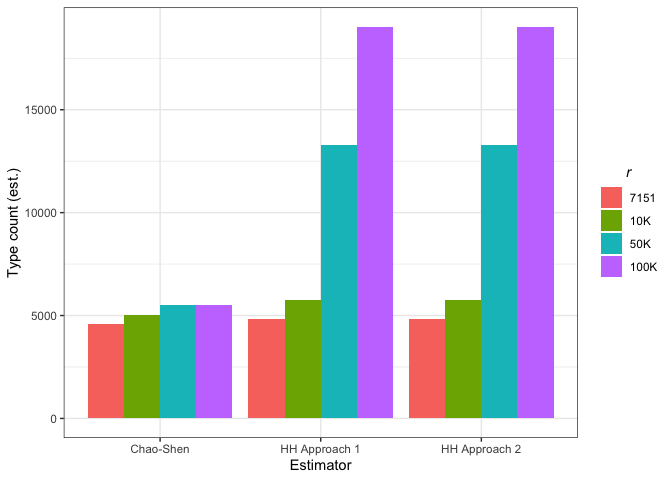
\includegraphics[width=0.8\linewidth]{README_files/figure-gfm/diff_plots_ext-1} 

}

\caption{\label{fig:diff_plot_ext}Type count estimates from the Chap and Herdan-Heaps' estimators for four sample sizes}\label{fig:diff_plot_ext}
\end{figure}

The two approaches to estimating \emph{n} for Herdan-Heaps are nearly
identical. Furthermore, we see diminishing rates of increase of the
estimates (going from 10K to 50K results in a greater increase than
going from 50K to 100K). For smaller \emph{r}, the Chao-Shen and
Herdan-Heaps' estimators behave similarly. As \emph{r} increases, the
degree of difference between the two estimators increases (as predicted
based on the underestimation bias reported above for Chao-Shen).

To summarize our main findings: (a) Herdan-Heaps' law fits the known
phonological diversity well, (b) a different strategy for estimating
type count performs best when it mimics Herdan-Heaps' law, (c) we
therefore have no reason to believe that there is a limit to the number
of phonemes to be observed in human languages, and (d) even if limited,
the true number is most likely much larger than what we have documented
so far.

\hypertarget{discussion}{%
\section{Discussion}\label{discussion}}

The present study asks a seemingly straightforward question: how many
different phonemes are possible in human language? We cannot determine
this number empirically from existing resources because the vast
majority of languages, known or unknown, are undocumented, extinct, or
both. Moreover, differences in documentary practice (theoretical and/or
methodological) mean that even our existing phonological descriptions
are provisional and objects of debate. For example, PHOIBLE contains
approximately 1.4 different inventories per language.\footnote{Different
  inventories per ``language'' mean they do not agree on the number or
  exact repertoire of phonemes. However, this should be expected given
  that phonological descriptions typically represent different
  doculects, i.e., different instances of linguistic behavior at
  different places, times, or with different speakers
  (\protect\hyperlink{ref-GoodCysouw2013}{Good \& Cysouw 2013}) and that
  phoneme analysis is a non-deterministic process
  (\protect\hyperlink{ref-Chao1934}{Chao 1934};
  \protect\hyperlink{ref-Hockett1963}{Hockett 1963}).}

To address these issues, we modeled the distributional properties of
documented phonemes. First, we found that frequencies of phoneme types
in existing cross-linguistic databases are well described by Zipf's law,
regardless of whether samples were controlled for areal and genetic
biases. Systems that obey Zipf's law, under mild assumptions, also
follow Herdan-Heaps' law
(\protect\hyperlink{ref-BaezaNavarro2000}{Baeza--Yates \& Navarro 2000};
\protect\hyperlink{ref-vanLeijenhorst2005}{Leijenhorst \& Van der Weide
2005}), which predicts type count from the number of tokens with only
two tunable parameters. Herdan-Heaps' law was originally intended to
describe how vocabulary size increases as more words are observed in a
document or set of documents. Extending this approach, we demonstrate
that the number of phoneme types in a sample of languages also grows
according to Herdan-Heaps' law. To our knowledge, we are the first to
apply Herdan-Heaps' law to the domain of segmental phonology by
reformulating it as estimator of the number of phonemes in groups of
languages. Finally, we verify the goodness-of-fit of Herdan-Heaps' by
applying an additional and formally unrelated tool borrowed from
ecology, which we refer to as the Chao-Shen estimator. The predictions
of this estimator confirm that the relationship between sample size and
segment type count is best described by a curve that approximates
Herdan-Heaps' law. Most importantly, the optimal Herdan-Heaps' model did
not converge on any single number of phoneme types as number of
languages increased.

Assuming a target of 7151 known languages,\footnote{\url{https://www.ethnologue.com/guides/how-many-languages}?}
our models predict a range of total segment types from 4592 to 4850
(mean = 4721). Based on PHOIBLE, our current best guess of the diversity
of documented phoneme types is 3183. Therefore, the models argue for the
existence of approximately 1500 yet to be documented phoneme types. As
we probe increasingly larger and theoretically motivated language sample
sizes, i.e., languages that existed \emph{through time} (e.g., estimates
including 30-500k (\protect\hyperlink{ref-Pagel2000}{Pagel 2000}) or
64-140k (\protect\hyperlink{ref-Crystal2002}{Crystal 2002})), the
Herdan-Heaps' model predicted a continual increase in the number of
unique phonemes, reaching values as high as 19k. The Chao-Shen model
produced much more conservative estimates for samples of size 10k and
above, even appearing to settle on an asymptote of roughly 5500 phonemes
for samples of 100k languages or more. However, when we compare the
predictions of Herdan-Heaps and Chao-Shen against known type counts in a
closed dataset, the source of the discrepancy emerged: as the sample
grows, Chao-Shen lags behind Herdan-Heaps in approximating the true
value. Thus, given a larger pool of training data, we expect Chao-Shen
to approximate more closely the estimates of Herdan-Heaps' law.

We therefore provisionally conclude three things: (1) adding languages
to a sample will always carry a non-zero probability of producing a
novel phoneme; (2) in accordance with Herdan-Heaps' law, the rate at
which new phonemes are discovered per language will always decrease; and
(3) the decrease in the rate of new observations will never reach 0.
Thus, based on the evidence presented here, we have no reason to believe
that there is an upper bound on the number of unique phonemes possible
in spoken languages. Infinite linguistic diversity seems to bring about
infinite possible phonemes. But what would it mean if there were indeed
infinitely many potential phonemes?

If one adopts a distinctive feature-based perspective on the phonetic
targets of phonemes, then there is an \emph{a priori} upper bound of
\(2^F\) contrastive sounds, where \(F\) is the number of feature
categories and 2 reflects the choice between presence (+) or absence (-)
of that feature.\footnote{In some distinctive feature sets, some values
  may be 0, i.e., undefined, underspecified, or ``for which a segment
  can be said `not to care''' (\protect\hyperlink{ref-Hayes2009}{Hayes
  2009}, pg. 91). For example, speech sounds that are -coronal are
  underspecified for the features +/-anterior and +/-distributed, which
  capture coronal distinctions for places of articulation involving
  (inter-)dentals and alveolars vs palatal alveolars and retroflexes
  (anterior), and laminal vs apical coronals (distributed).} Clements
(\protect\hyperlink{ref-Clements2009}{2009}) coined this calculation
\emph{Feature Bounding}. The expected number of unique phonemes is
controlled by the number of features, where additional features increase
the pool of possible distinctive segments (nearly) exponentially. For
example, given a feature set such as in PHOIBLE with 37 distinctive
features, an upper bound on the number of segments under a strictly
binary formalization is over 137 billion (2\^{}37) feature vectors. In
general, distinctive feature theories of different theoretical stances
propose around two dozen features
(\protect\hyperlink{ref-MielkeHume2006}{Mielke \& Hume 2006}), which
still has the potential to generate over 16 million distinct feature
vectors (2\^{}24). Crucially, this theoretical bound on phoneme
diversity does not in itself preclude the possibility of infinitely many
phonemes. To get there, one would only need to discover infinitely many
distinctive features. But, as pointed out by Lindblom
(\protect\hyperlink{ref-Lindblom1990a}{1990}), most proponents of
feature-based analysis assume a fixed, small-ish inventory of features.
The question would then be: how does the feature pool grow empirically
with the addition of new languages? Does it converge as assumed?
Unfortunately, this question presents a host of new challenges, not the
least of which concerns how to define the features themselves.

Most widely accepted feature sets define features that are specified at
different levels of phonetic detail: some features are more abstract
(i.e., general similarities such as +/- syllabic), while others are more
concrete (i.e., closer to the articulatory reality, e.g., advanced
tongue root). Some are grounded in pure articulatory or acoustic
phonetics, while others involve phonological properties of language. And
looming in the background of these discussions, the debate of whether
distinctive features are innate and universal or rather learned and
emergent continues. Thus, the precise limits on what may be included as
a feature are underspecified and a matter of some controversy (for more
fundamental critiques of features and how they are defined, see Lindblom
(\protect\hyperlink{ref-Lindblom1990a}{1990})). Current consensus and
critiques aside, there does not appear to be a principled limit to the
degree of phonetic specificity that can be encoded by a feature. Making
finer and finer contrasts may always produce more and more features.
Thus, the exponent in the Feature Bounding calculation can itself (by
hypothesis) be infinite, in line with the predictions of the models
presented here, and therefore with the notion of infinite possible
phonemes. That said, contemporary feature sets can capture phonological
classes for place and manner of articulation, which neatly classify the
phonological patterns and processes in and across languages (cf. Mielke
(\protect\hyperlink{ref-Mielke2008}{2008})).

We have so far seen that the feature space is a discrete re-coding of
the continuous variability of the physical acoustic and articulatory
spaces -- and so it should by way of finer and finer specification, be
able to support an infinitely diverse set of phonemes. However, one
objection to this account is that humans are subject to physiological
limits, both in production and perception. In speech production,
articulatory gestures are executed with some degree of imprecision
(\protect\hyperlink{ref-Ladefoged_etal1972}{Ladefoged et al. 1972};
\protect\hyperlink{ref-LindblomSundberg1971}{Lindblom \& Sundberg
1971}). If this stochastic variability is greater than the difference
between two or more phonetic targets, then no reliable distinction can
be sustained (cf. Stevens (\protect\hyperlink{ref-Stevens1972}{1972})).
In comparison, if the range of articulatory gestures is greater than
their acoustic (or perceptual) reception, there is a ``many-to-one''
mapping between articulation and perception. In perception, the ability
to discriminate acoustic stimuli is also limited both anatomically and
cognitively. Differences in the signal that fall below the various
thresholds for discrimination are thus ignored.

In response to these physical constraints, languages tend to spread
their phonological inventories across the articulatory and acoustic
spaces, thereby maintaining workable discriminability. A stark example
comes from Central Rotokas (North Bougainville; Papua New Guinea), which
has only 6 consonants (9 counting allophones) from three easily
discriminated places of articulation: labials \texttt{{[}p,\ b{]}},
alveolars \texttt{{[}t,\ d{]}}, and velars \texttt{{[}k,\ g{]}}
(\protect\hyperlink{ref-FirchowFirchow1969}{Firchow \& Firchow 1969}).
Compare this to a hypothetical less-optimal language that contrasts only
\texttt{{[}t,\ d{]}}, \texttt{{[}tʰ,\ dʰ{]}}, and \texttt{{[}t̪,\ d̪{]}}.
Given this strategy, it is unlikely that ultra-fine-grained phonetic
contrasts would ever arise in a single language. Rather, the contrasts
are most likely to arise between languages. In other words, the infinity
of phonemes predicted by the analyses reported here plays out in the
realm of cross-linguistic variation of phonetic targets, even if those
differences cannot be reliably articulated by a single tongue or
perceived by a single ear.

Given that all speakers use perceptually contrastive cues (whether
signed, spoken or written), how these continuous signals map to discrete
elements is a core question of language science that goes beyond what
the phonetics-phonology interface may or may not be. Thus, we believe
the approaches presented here have broad applications to the study of
other areas of grammar and to the cross-linguistic study of languages.

\hypertarget{data-accessibility}{%
\section{Data accessibility}\label{data-accessibility}}

Data and code required to reproduce all results presented in this paper
are available as electronic supplementary material at:
\url{https://github.com/bambooforest/heaps}.

\hypertarget{competing-interests}{%
\section{Competing interests}\label{competing-interests}}

The authors declare no competing interests.

\hypertarget{acknowledgements}{%
\section{Acknowledgements}\label{acknowledgements}}

SM was funded by the Swiss National Science Foundation (Grant
No.~PCEFP1\_186841).

\hypertarget{author-contributions}{%
\section{Author contributions}\label{author-contributions}}

SM conceptualization. SM and NAL designed the study, interpreted the
results, and wrote the paper.

\hypertarget{references}{%
\section*{References}\label{references}}
\addcontentsline{toc}{section}{References}

\hypertarget{refs}{}
\begin{CSLReferences}{1}{0}
\leavevmode\vadjust pre{\hypertarget{ref-BaezaNavarro2000}{}}%
Baeza--Yates, Ricardo \& Gonzalo Navarro. 2000. Block addressing indices
for approximate text retrieval. \emph{Journal of the American Society
for Information Science} 51(1). 69--82.

\leavevmode\vadjust pre{\hypertarget{ref-Boersma2001}{}}%
Boersma, Paul. 2001. Praat, a system for doing phonetics by computer.
\emph{Glot International} 5. 341--345.

\leavevmode\vadjust pre{\hypertarget{ref-BrantsFranz2006}{}}%
Brants, Thorsten \& Alex Franz. 2006. {Web 1T 5-gram Version 1 (2006)}.
\emph{Linguistic Data Consortium, Philadelphia}.

\leavevmode\vadjust pre{\hypertarget{ref-ChaoChiu2016}{}}%
Chao, Anne \& Chun-Huo Chiu. 2016. Species richness: Estimation and
comparison. In \emph{{Wiley StatsRef: Statistics Reference Online}},
1--26. John Wiley \& Sons.

\leavevmode\vadjust pre{\hypertarget{ref-Chao_etal2009}{}}%
Chao, Anne, Robert K Colwell, Chih-Wei Lin \& Nicholas J Gotelli. 2009.
Sufficient sampling for asymptotic minimum species richness estimators.
\emph{Ecology}. Wiley Online Library 90(4). 1125--1133.

\leavevmode\vadjust pre{\hypertarget{ref-Chao1934}{}}%
Chao, Yuen-ren. 1934. The non-uniqueness of phonemic solutions of
phonetic systems. \emph{Academia Sinica (Bulletin of the Institute of
History and Philology)} 4(4).

\leavevmode\vadjust pre{\hypertarget{ref-Clements2009}{}}%
Clements, G. N. 2009. The role of features in phonological inventories.
In Eric Raimy \& Charles E. Cairns (eds.), \emph{Contemporary views on
architecture and representations in phonology}, 19--68. MIT Press.

\leavevmode\vadjust pre{\hypertarget{ref-Crystal2002}{}}%
Crystal, David. 2002. \emph{Language death}. Cambridge University Press.

\leavevmode\vadjust pre{\hypertarget{ref-Egghe2007}{}}%
Egghe, Leo. 2007. Untangling {Herdan's} law and {Heaps'} law:
Mathematical and informetric arguments. \emph{Journal of the American
Society for Information Science and Technology} 58(5). 702--709.

\leavevmode\vadjust pre{\hypertarget{ref-EvansLevinson2009}{}}%
Evans, Nicholas \& Stephen C. Levinson. 2009. The myth of language
universals: Language diversity and its importance for cognitive science.
\emph{Behavioral and Brain Sciences} 32(5). 429--448.

\leavevmode\vadjust pre{\hypertarget{ref-Everett2018}{}}%
Everett, Caleb. 2018. The similar rates of occurrence of consonants
across the world's languages: A quantitative analysis of phonetically
transcribed word lists. \emph{Language Sciences} 69. 125--135.

\leavevmode\vadjust pre{\hypertarget{ref-FirchowFirchow1969}{}}%
Firchow, Irwin \& Jacqueline Firchow. 1969. An abbreviated phoneme
inventory. \emph{Anthropological Linguistics} 11. 271--276.

\leavevmode\vadjust pre{\hypertarget{ref-GoodCysouw2013}{}}%
Good, Jeff \& Michael Cysouw. 2013. Languoid, doculect, and glossonym:
Formalizing the notion {``language.''} \emph{Language Documentation \&
Conservation} 7. 331--359.

\leavevmode\vadjust pre{\hypertarget{ref-Hayes2009}{}}%
Hayes, Bruce. 2009. \emph{Introductory phonology}. Blackwell.

\leavevmode\vadjust pre{\hypertarget{ref-Heaps1978}{}}%
Heaps, Harold Stanley. 1978. \emph{Information retrieval, computational
and theoretical aspects}. Academic Press.

\leavevmode\vadjust pre{\hypertarget{ref-Herdan1964}{}}%
Herdan, Gustav. 1964. \emph{Quantitative linguistics}. London:
Butterworth.

\leavevmode\vadjust pre{\hypertarget{ref-Hockett1963}{}}%
Hockett, Charles. 1963. The problem of universals in language. In Joseph
H. Greeberg (ed.), \emph{Universals of language}. Cambridge, MA: MIT
Press.

\leavevmode\vadjust pre{\hypertarget{ref-Hockett1995-phoneme}{}}%
Hockett, Charles F. 1995. The birth and deaths of the phoneme.
\emph{Id{é}ologies dans le Monde Anglo-Saxon} 8. 5--50.

\leavevmode\vadjust pre{\hypertarget{ref-Joos1948}{}}%
Joos, Martin. 1948. Acoustic phonetics. \emph{Language} 24(2). 5--136.

\leavevmode\vadjust pre{\hypertarget{ref-JustesonStephens1984}{}}%
Justeson, John S. \& Laurence D. Stephens. 1984. On the relationship
between the numbers of vowels and consonants in phonological systems.
\emph{Linguistics} 22. 531--545.

\leavevmode\vadjust pre{\hypertarget{ref-Kornai2002}{}}%
Kornai, András. 2002. {How many words are there?} \emph{Glottometrics}
4. 61--86.

\leavevmode\vadjust pre{\hypertarget{ref-Ladefoged_etal1972}{}}%
Ladefoged, Peter, Joseph DeClerk, Mona Lindau \& George Papcun. 1972. An
auditory-motor theory of speech production. \emph{{UCLA} working papers
in phonetics} 22(48). 48--76.

\leavevmode\vadjust pre{\hypertarget{ref-Lehfeldt1975}{}}%
Lehfeldt, Werner. 1975. {Die Verteilung der Phonemanzahl in den
nat{ü}rlichen Sprachen}. \emph{Phonetica} 31. 247--287.

\leavevmode\vadjust pre{\hypertarget{ref-vanLeijenhorst2005}{}}%
Leijenhorst, Dick C van \& Th P Van der Weide. 2005. A formal derivation
of {Heaps'} law. \emph{Information Sciences} 170(2-4). 263--272.

\leavevmode\vadjust pre{\hypertarget{ref-Lindblom1990a}{}}%
Lindblom, Björn. 1990. On the notion of {``possible speech sound.''}
\emph{Journal of Phonetics} 18(2). 135--152.

\leavevmode\vadjust pre{\hypertarget{ref-LindblomSundberg1971}{}}%
Lindblom, Björn \& Johan Sundberg. 1971. Acoustical consequences of lip,
tongue, jaw, and larynx movement. \emph{The Journal of the Acoustical
Society of America} 50(4B). 1166--1179.

\leavevmode\vadjust pre{\hypertarget{ref-Macklin-CordesRound2020}{}}%
Macklin-Cordes, Jayden L \& Erich R Round. 2020. Re-evaluating phoneme
frequencies. \emph{Frontiers in Psychology} 11. 570895.

\leavevmode\vadjust pre{\hypertarget{ref-Maddieson1984}{}}%
Maddieson, Ian. 1984. \emph{Patterns of sounds}. Cambridge: Cambridge
University Press.

\leavevmode\vadjust pre{\hypertarget{ref-Maddieson2008}{}}%
Maddieson, Ian. 2008. Consonant inventories. In Martin Haspelmath,
Matthew S. Dryer, David Gil \& Bernard Comrie (eds.), \emph{The world
atlas of language structures online}. Munich: Max Planck Digital
Library.

\leavevmode\vadjust pre{\hypertarget{ref-MaddiesonPrecoda1990}{}}%
Maddieson, Ian \& Kristin Precoda. 1990. {Updating UPSID}. In \emph{UCLA
working papers in phonetics}, vol. 74, 104--111. Department of
Linguistics, UCLA.

\leavevmode\vadjust pre{\hypertarget{ref-Martindale_etal1996}{}}%
Martindale, Colin, S. M. Gusein-Zade, Dean McKenzie \& Mark Yu.
Borodovsky. 1996. Comparison of equations describing the ranked
frequency distributions of graphemes and phonemes. \emph{Journal of
Quantitative Linguistics} 3(2). 106--112.

\leavevmode\vadjust pre{\hypertarget{ref-Mielke2008}{}}%
Mielke, Jeff. 2008. \emph{{The Emergence of Distinctive Features}}.
Oxford University Press.

\leavevmode\vadjust pre{\hypertarget{ref-MielkeHume2006}{}}%
Mielke, Jeff \& Elizabeth Hume. 2006. Distinctive features. In
\emph{{Encylopedia of Langauge}}. Elsevier.

\leavevmode\vadjust pre{\hypertarget{ref-Milivcka2009}{}}%
Milička, Jiři. 2009. Type-token \& hapax-token relation: A combinatorial
model. \emph{Glottotheory} 2(1). 99--110.

\leavevmode\vadjust pre{\hypertarget{ref-Moran2012}{}}%
Moran, Steven. 2012. \emph{{Phonetics Information Base and Lexicon}}.
University of Washington PhD thesis.

\leavevmode\vadjust pre{\hypertarget{ref-MoranMcCloy2019}{}}%
Moran, Steven \& Daniel McCloy (eds.). 2019. \emph{{PHOIBLE 2.0}}. Jena:
Max Planck Institute for the Science of Human History.

\leavevmode\vadjust pre{\hypertarget{ref-Pagel2000}{}}%
Pagel, Mark. 2000. The history, rate and pattern of world linguistic
evolution. In Chris Knight, Michael Studdert-Kennedy \& James Hurford
(eds.), \emph{The evolutionary emergence of language: Social function
and the origins of linguistic form}, 391--416. Cambridge University
Press.

\leavevmode\vadjust pre{\hypertarget{ref-Piantadosi2014}{}}%
Piantadosi, Steven T. 2014. Zipf's word frequency law in natural
language: A critical review and future directions. \emph{Psychonomic
Bulletin \& Review} 21(5). 1112--1130.

\leavevmode\vadjust pre{\hypertarget{ref-Potter1945}{}}%
Potter, Ralph K. 1945. Visible patterns of sound. \emph{Science}
102(2654). 463--470.

\leavevmode\vadjust pre{\hypertarget{ref-Snyman1970}{}}%
Snyman, J. W. 1970. \emph{{An Introduction to the !Xu (!Kung)
Language}}. Capetown: A. A. Balkema.

\leavevmode\vadjust pre{\hypertarget{ref-Snyman1975}{}}%
Snyman, J. W. 1975. \emph{{Zu\textbar'hoasi Fonologie en Woordeboek}}.
Cape Town: A. A. Balkema.

\leavevmode\vadjust pre{\hypertarget{ref-Stevens1972}{}}%
Stevens, Kenneth N. 1972. The quantal nature of speech: Evidence from
articulatory-acoustic data. In Edward E David \& Peter B Denes (eds.),
\emph{Human communication: A unified view}. New York: McGraw-Hill.

\leavevmode\vadjust pre{\hypertarget{ref-TambovtsevMartindale2007}{}}%
Tambovtsev, Yuri \& Colin Martindale. 2007. Phoneme frequencies follow a
{Yule} distribution. \emph{SKASE Journal of Theoretical Linguistics}
4(2). 1--11.

\leavevmode\vadjust pre{\hypertarget{ref-Whalen2019}{}}%
Whalen, Douglas H. 2016. Phonetics. In \emph{Oxford research
encyclopedia of linguistics}. Oxford University Press.

\leavevmode\vadjust pre{\hypertarget{ref-Zipf1936}{}}%
Zipf, George Kingsley. 1936. \emph{The psychobiology of language}.
London: Routledge.

\leavevmode\vadjust pre{\hypertarget{ref-Zipf1949}{}}%
Zipf, George Kingsley. 1949. \emph{Human behavior and the principle of
least effort}. New York: Addison-Wesley.

\end{CSLReferences}

\end{document}
